\section{BANENOR}
\label{res:Judas}


\subsection{Experiment \rnum{1}: HDF5 file processing and resampling}

\begin{figure}[!h]
    \centering
    \begin{subfigure}{0.45\linewidth}
        \centering
        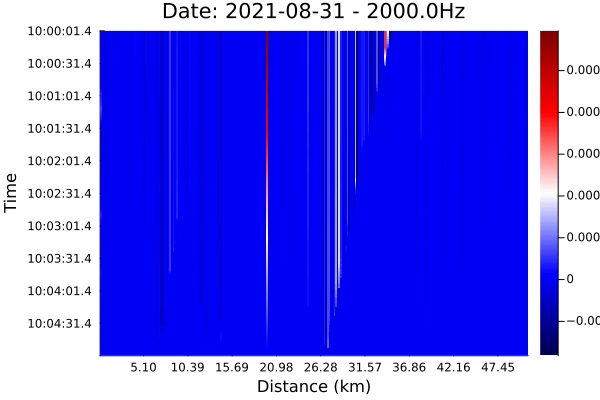
\includegraphics[width=\linewidth]{figures/heatmap_das_test.png}
        \caption{Before resampling and normalization}
        \label{fig:dasoutput1}
    \end{subfigure}
    \hfill
    \begin{subfigure}{0.45\linewidth}
        \centering
        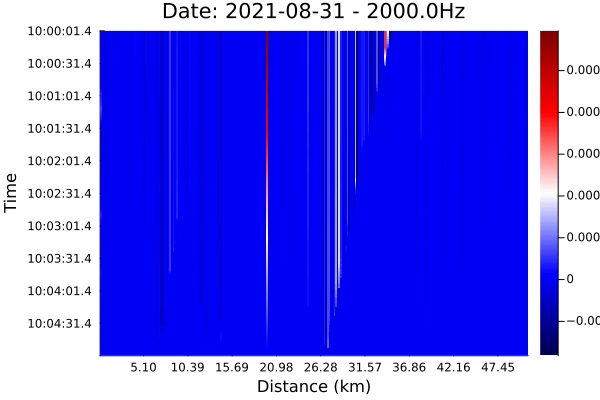
\includegraphics[width=\linewidth]{figures/heatmap_das_test.png}
        \caption{After resampling and normalization}
        \label{fig:dasoutput2}
    \end{subfigure}
    \caption{Heatmaps of the processed data before and after }
    \label{fig:dasoutput}
\end{figure}
\begin{figure}[!htbp]
\centering
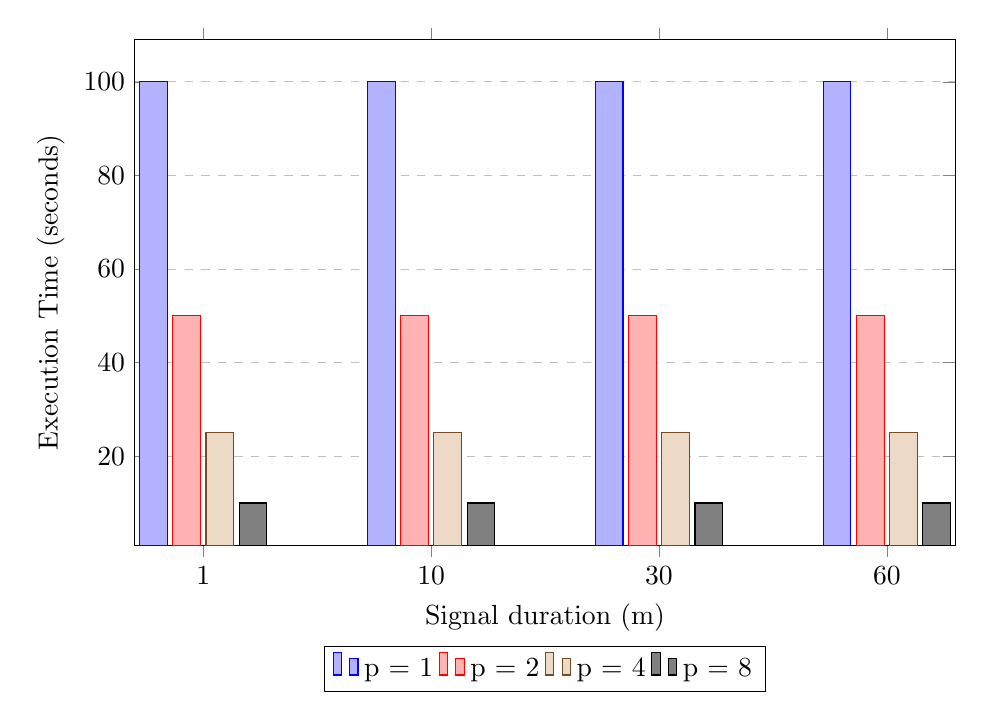
\begin{tikzpicture}
\begin{axis}[
    ylabel={Execution Time (seconds)},
    xlabel={Signal duration (m)},
    xticklabels={1,10, 30, 60},
    xtick={1,10,30,60},
    legend pos=north west,
    ymajorgrids=true,
    grid style=dashed,
    width=12cm,
    height=8cm,
    bar width=10pt,
    ybar,
    legend style={at={(0.5,-0.20)},
    anchor=north,legend columns=-1},
    symbolic x coords={1, 10, 30, 60},
]
\addplot coordinates {(1,100)(10,100)(30,100)(60,100) };
\addplot coordinates {(1,50) (10,50) (30,50) (60,50) };
\addplot coordinates {(1,25) (10,25) (30,25) (60,25) };
\addplot coordinates {(1,10) (10,10) (30,10) (60,10) };
\legend{p = 1, p = 2, p = 4, p = 8}
\end{axis}
\end{tikzpicture}
\caption{Execution times for different problem sizes and process counts}
\label{fig:judas-benchmark}
\end{figure}

As we can see.

\begin{figure}[!htbp]
\centering
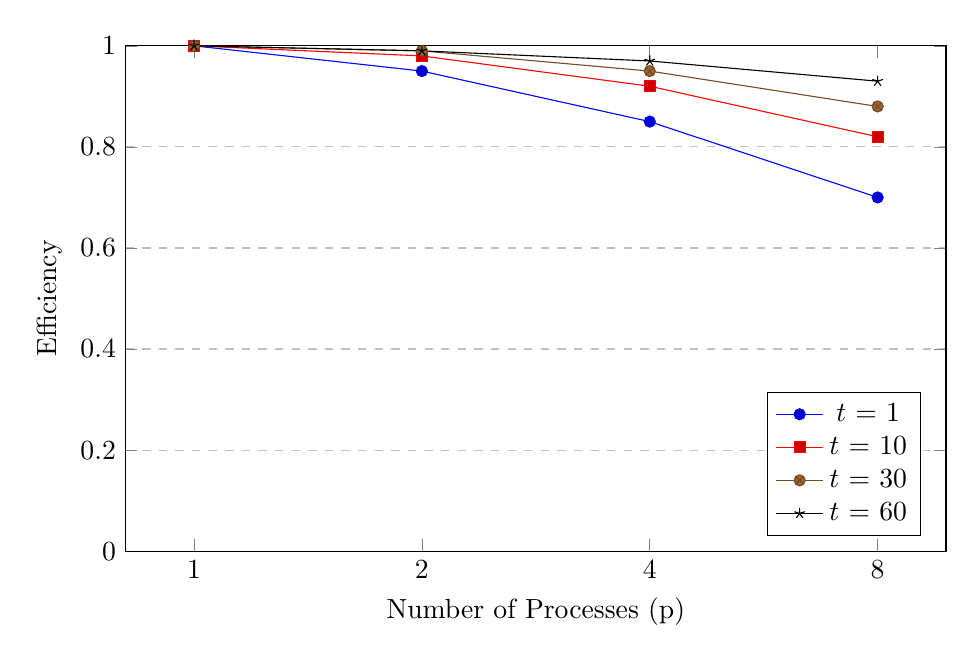
\begin{tikzpicture}
\begin{axis}[
    ylabel={Efficiency},
    xlabel={Number of Processes (p)},
    xticklabels={1,2,4,8},
    xtick={1,2,3,4},
    legend pos=south east,
    ymajorgrids=true,
    grid style=dashed,
    width=12cm,
    height=8cm,
    ymax=1,
    ymin=0,
]
\addplot coordinates {(1,1) (2,0.95) (3,0.85) (4,0.70)};
\addplot coordinates {(1,1) (2,0.98) (3,0.92) (4,0.82)};
\addplot coordinates {(1,1) (2,0.99) (3,0.95) (4,0.88)};
\addplot coordinates {(1,1) (2,0.99) (3,0.97) (4,0.93)};
\legend{$t$ = 1, $t$ = 10, $t$ = 30, $t$ = 60}
\end{axis}
\end{tikzpicture}
\caption{Efficiency for different problem sizes and process counts. $m$ is the amount of minutes of data we want to process.}
\label{fig:efficiency}
\end{figure}

\subsection{Experiment \rnum{2}: Parallel Resampling}

\begin{figure}[!htbp]
\centering
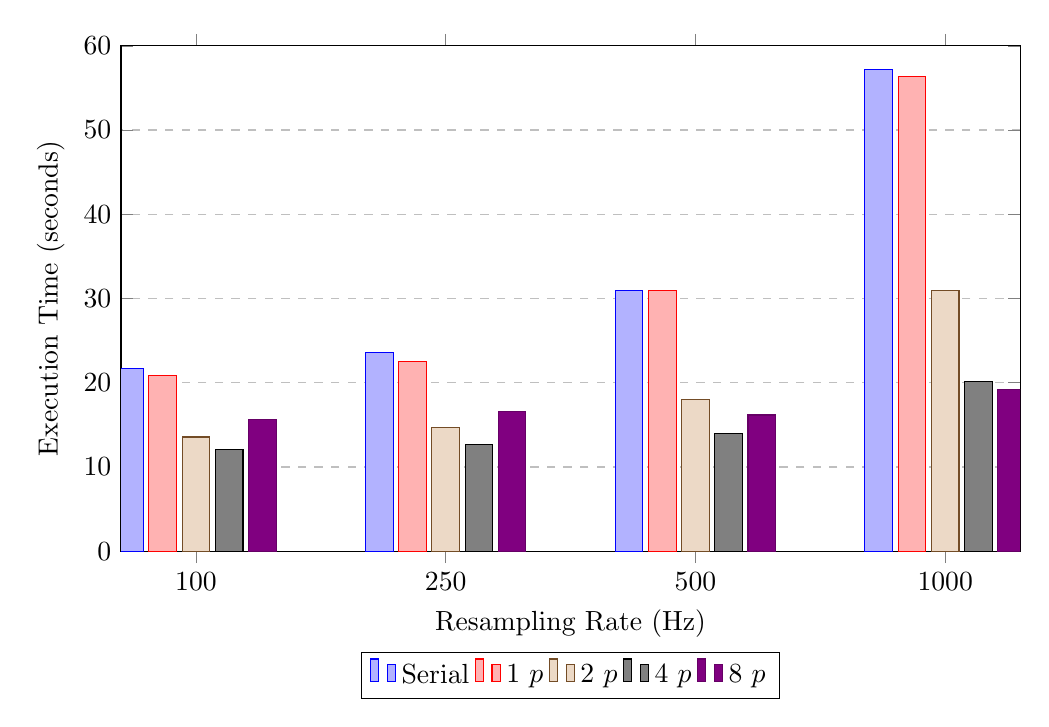
\begin{tikzpicture}
\begin{axis}[
    ylabel={Execution Time (seconds)},
    xlabel={Resampling Rate (Hz)},
    xticklabels={1000, 500, 250, 100},
    xtick={1000,500,250,100},
    legend pos=north west,
    ymajorgrids=true,
    grid style=dashed,
    width=13cm,
    height=8cm,
    bar width=10pt,
    ybar,
    legend style={at={(0.5,-0.20)},
    anchor=north,legend columns=-1},
    symbolic x coords={1000, 500, 250, 100},
    x dir=reverse,
    ymin=0, ymax=60,
]
\addplot coordinates {(1000,57.205) (500,30.970) (250,23.580) (100,21.695)};
\addplot coordinates {(1000,56.351) (500,30.941) (250,22.491) (100,20.843)};
\addplot coordinates {(1000,30.956) (500,17.998) (250,14.719) (100,13.556)};
\addplot coordinates {(1000,20.125) (500,13.937) (250,12.698) (100,12.066)};
\addplot coordinates {(1000,19.217) (500,16.173) (250,16.604) (100,15.619)};
\legend{Serial, 1 $p$, 2 $p$, 4 $p$, 8 $p$}
\end{axis}
\end{tikzpicture}
\caption{Execution times for different resampling rates and process counts $p$}
\label{fig:resampling-benchmark}
\end{figure}

\begin{figure}[!h]
    \centering
    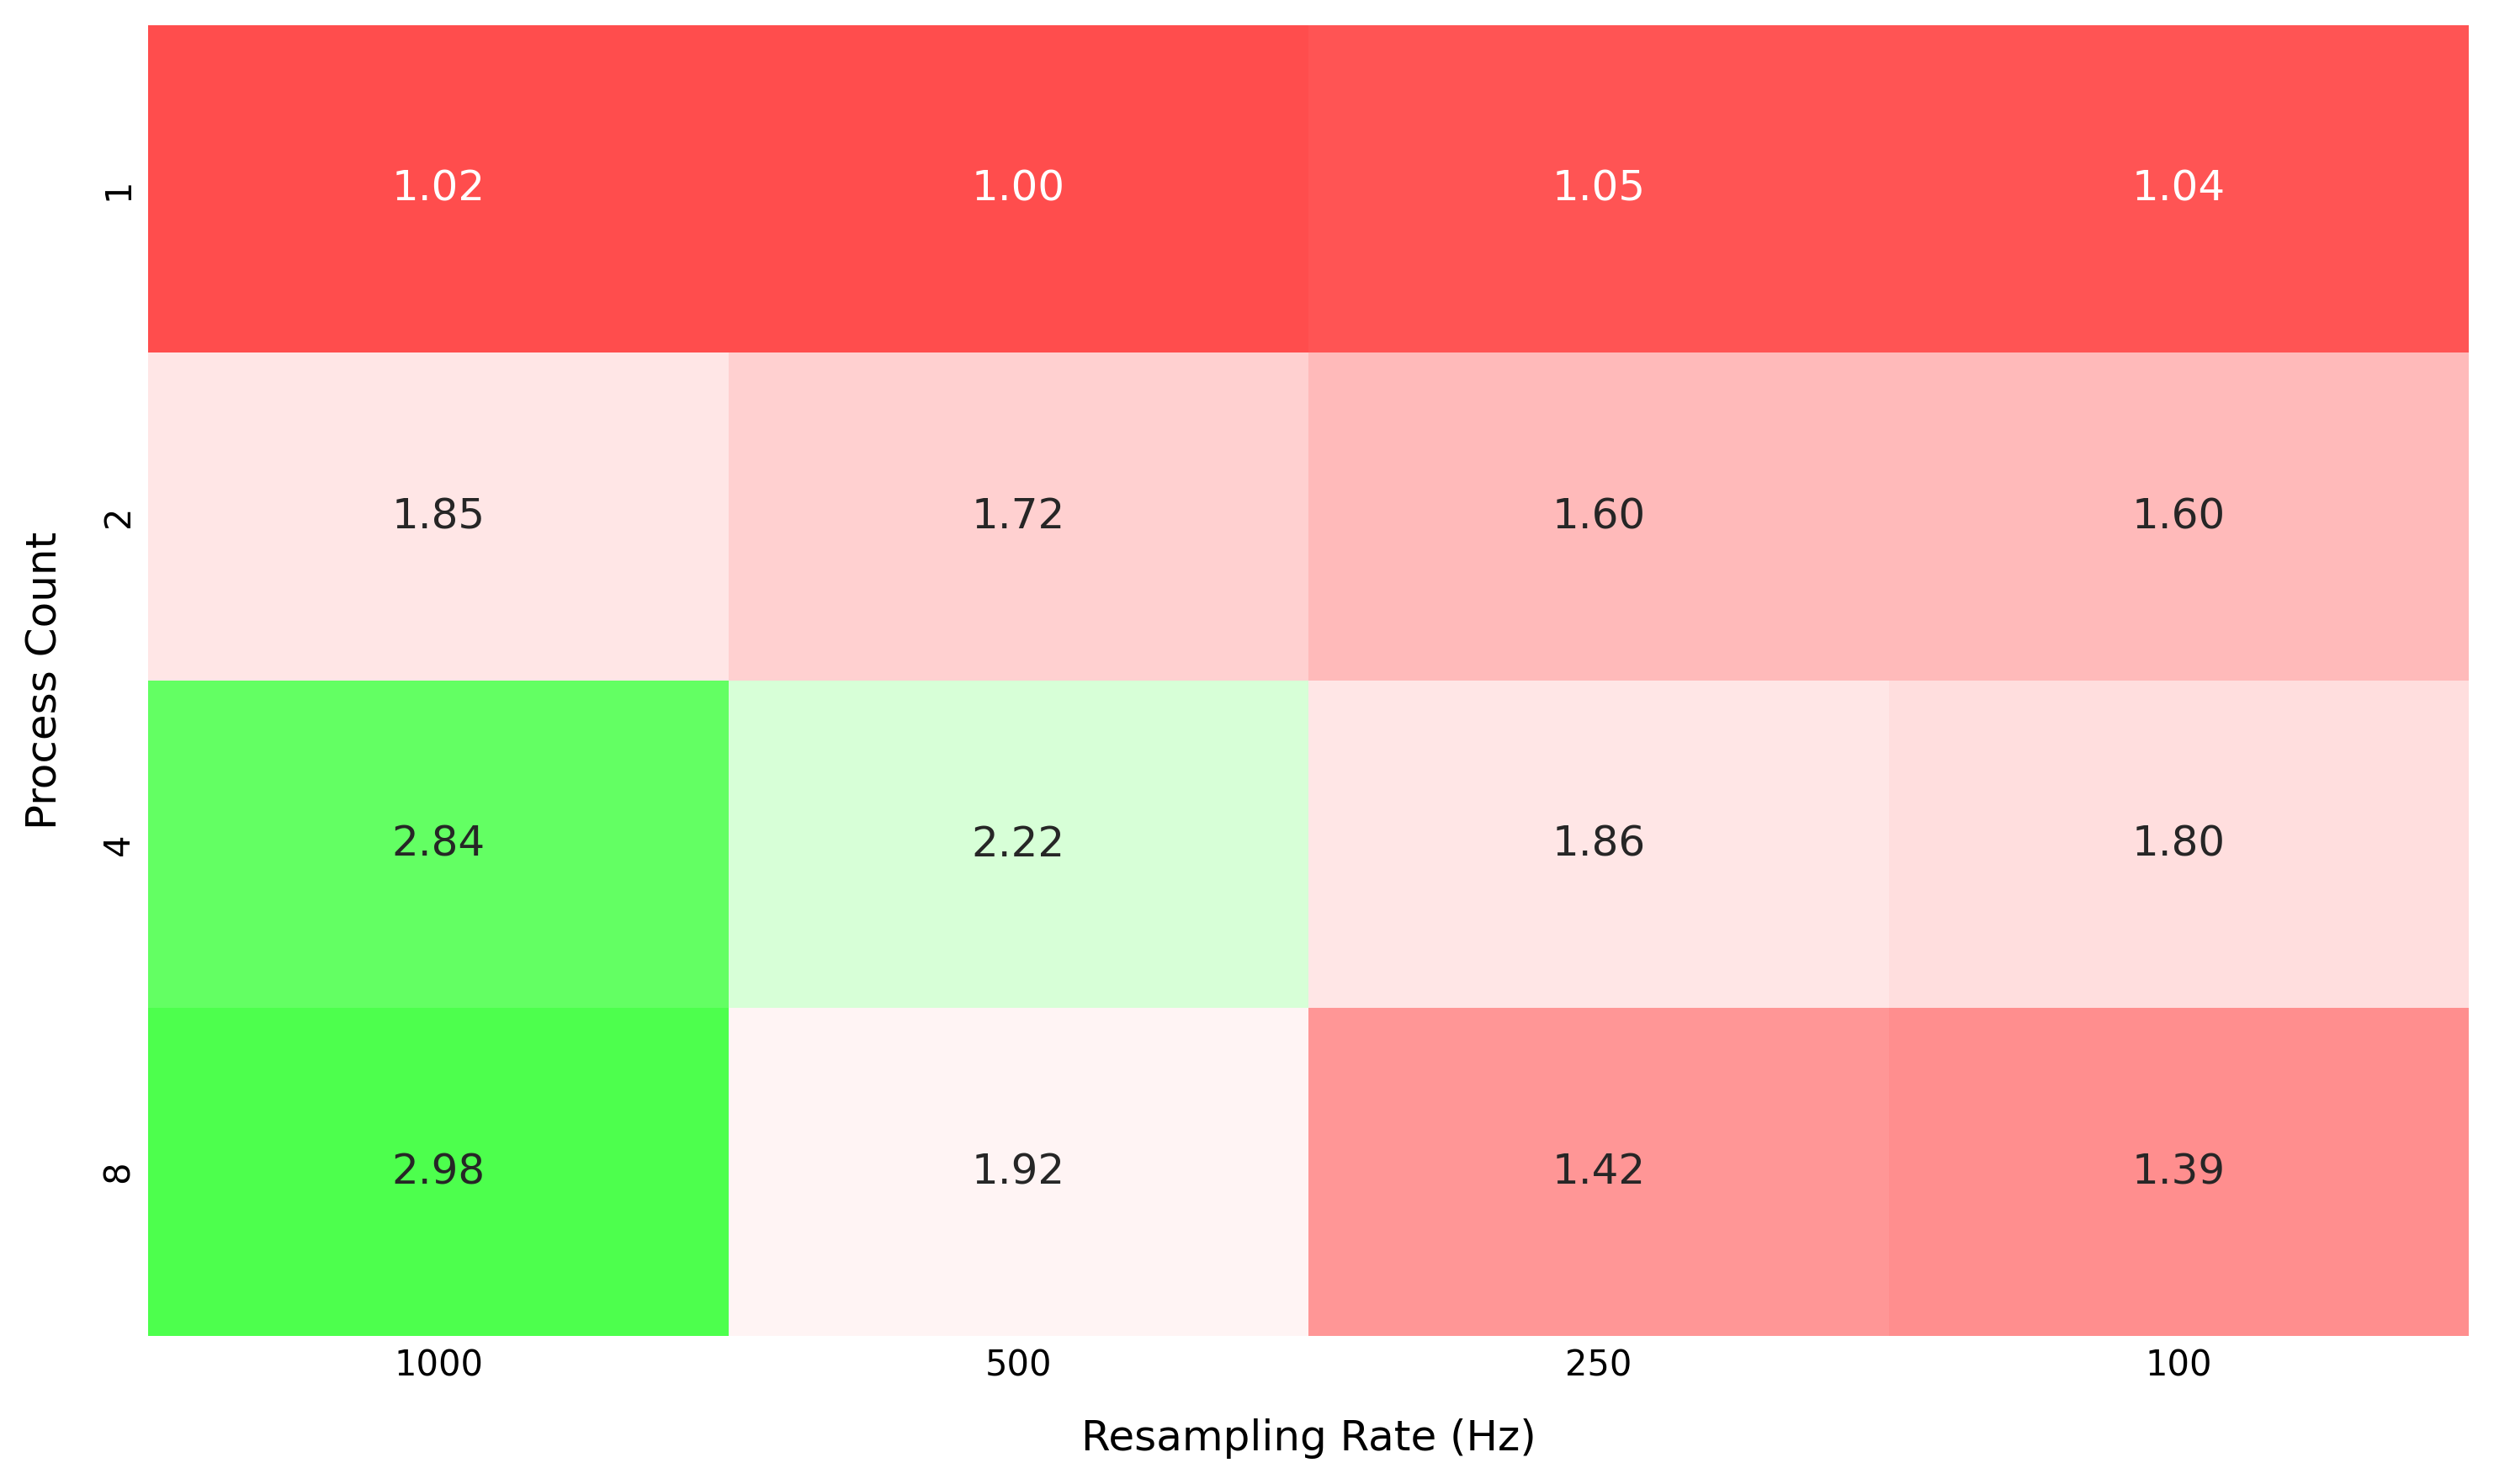
\includegraphics[scale=0.5]{figures/speedup_heatmap(1).png}
    \caption{Heatmap of speedups compared to serial execution}
    \label{fig:ex2heat}
\end{figure}

\begin{figure}[!htbp]
\centering
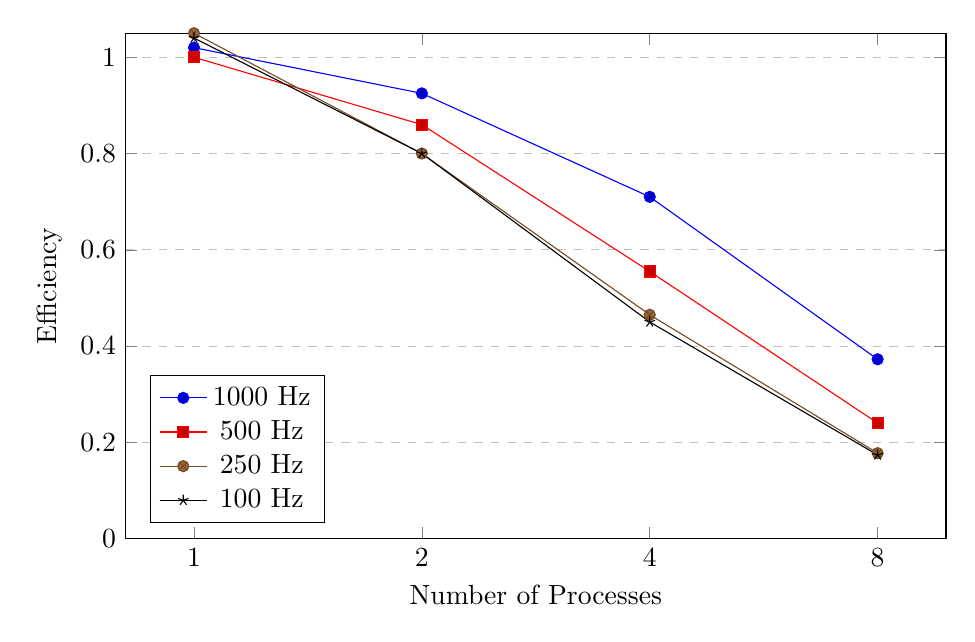
\begin{tikzpicture}
\begin{axis}[
    ylabel={Efficiency},
    xlabel={Number of Processes},
    xticklabels={1,2,4,8},
    xtick={1,2,3,4},
    legend pos=south west,
    ymajorgrids=true,
    grid style=dashed,
    width=12cm,
    height=8cm,
    ymax=1.05,
    ymin=0,
]
\addplot coordinates {(1,1.02) (2,0.925) (3,0.71) (4,0.3725)};
\addplot coordinates {(1,1.00) (2,0.86) (3,0.555) (4,0.24)};
\addplot coordinates {(1,1.05) (2,0.80) (3,0.465) (4,0.1775)};
\addplot coordinates {(1,1.04) (2,0.80) (3,0.45) (4,0.17375)};
\legend{1000 Hz, 500 Hz, 250 Hz, 100 Hz}
\end{axis}
\end{tikzpicture}
\caption{Efficiency for different resampling rates and process counts}
\label{fig:resampling_efficiency}
\end{figure}


